\chapter{Mission analysis}
\qquad \underline{By} : Tim
\section{Mission Summary}
The objective of the mission is the deorbiting of a GEO satellite. The first step to developing the
propulsion system is to break down the mission segments and calculate the delta-V for each of them.
Then after the $\Delta v$ and some mission constraints are clear the detailed mission profile needs to be chosen and optimized.\\

The mission is broken down into two major phases. Phase 1 is to reach the satellites orbit and match its
velocity to enable the capturing process. Phase 2 is deorbiting the satellite and retuning to the original LEO orbit.
\subsection{Phase 1}
\begin{center}
	Transferring the spacecraft from LEO at $55^\circ$ inclination to GEO at $0^\circ$ inclination
\end{center}
First concept : \\

\begin{itemize}
	\item Burn 1.1 : LEO to GTO at $55^\circ$
	\item Burn 1.2 : Inclination change to $0^\circ$ at Apogee of GTO
	\item Burn 1.3 : GTO to GEO at $0^\circ$
\end{itemize}
To calculate the required delta-V for a burn to change the velocity without changing the direction of the spacecraft is simply identifying the difference in value of the starting and target vector. So for Burn 1.1 the orbital speed of LEO at 400 km needs to be calculated as well as the perigee speed of an elliptic orbit with 400 km as perigee and GEO altitude as apogee. To calculate these values several Matlab functions were written:

\begin{minted}[fontsize=\footnotesize, linenos, autogobble, breaklines]{matlab}
function a = v(r) % velocity of a circular orbit with Radius r
a = sqrt(mu/r);
end
\end{minted}
Then the function was used for the calculation with $R_{LEO} = 6778$ km
\begin{equation}
	v_{LEO} = v(R_{LEO}) = 7669 m/s
\end{equation}
The target velocity for the perigee of the GTO is calculated with the following function:
\begin{minted}[fontsize=\footnotesize, linenos, autogobble, breaklines]{matlab}
function a = vp(r, R) % perigee velocity of elliptical orbit with perigee r and apogee R
if r<R %if clause to prevent mistaken input
a = sqrt(2*mu/r-2*mu/(r+R));
end
end
\end{minted}

With $R_{GEO} = 42164$ km, the speed is calculated:
\begin{equation}
	v_{gto_p} = v_p(R_leo, R_geo) = 10066 m/s
\end{equation}
The difference between the two values is the required $\Delta v, \Delta v_1 = 2398$ m/s.\\

To calculate the delta-V needed for an inclination change the following function was used:
\begin{minted}[fontsize=\footnotesize, linenos, autogobble, breaklines]{matlab}
function a= dVi(i, v) % delta-V required for inclination change of i (deg) and velocity v
a= 2*v*sin(deg2rad(i)/2);
end
\end{minted}

The velocity passed to the function is the velocity at which the inclination change shall be performed.
Here the apogee velocity of the GTO $v_{gto_a} = 1618$ m/s was used:
\begin{equation}
	\Delta v{inc_1} = \Delta v_i(i, v_{gto_a})
\end{equation}

Lastly, the velocity change from the apogee of the GTO $v_{gto_a}$ and the velocity at GEO $v_{geo} = 3075 m/s$ needs to be calculated. The difference between the two values is $\Delta v_2 = 1457$ m/s.\\

Now all the three delta-Vs are added to the delta-V requirement of phase 1:
\begin{equation}
	\Delta v_{phase_1} = \Delta v_1+\Delta v_1+\Delta v_{inc1} = 5348 m/s
\end{equation}


\subsection{Phase 2 }
\begin{center}
	Transferring the captured satellite to a deorbiting trajectory and returning to LEO at $55^\circ$ inclination
\end{center}
First concept : \\


After capture the satellite needs to be deorbited. Herefore it needs to be set to a drop trajectory. But
since the spacecraft shall not deorbit but stay in LEO it needs to make short correction burn to slightly increase the targeted perigee.
\begin{itemize}
	\item Burn 2.1 : GEO to GTO with (with DROP altitude as perigee, afterwards detaching the satellite)
	\item Burn 2.2 : Inclination change to $55^\circ$
	\item Burn 2.3 : GTO(DROP) to GTO(LEO as perigee)
	\item Burn 2.4 : GTO(LEO) to LEO
\end{itemize}
These $\Delta v$ are calculated in the same way as described above. The total $\Delta v$ for phase 2 with $v_{drop_a} = 1587$ m/s, $v_{aero_{a1}} = 1592$ m/s, $v_{aero_{p1}} = 10283$ m/s, $v_{lto_p}
= 7887$ m/s and $v_{lto_a} = 7596$ m/s.

\begin{align}
	\Delta v_3 &=\Delta v(v_{GEO}, v_{drop_a}) = 1488 m/s\\
	\Delta v_4 &=\Delta v(v_{drop_a}, v_{aero_{a1}}) = 5 m/s   \\
	\Delta v_5 &=\Delta v(v_{aero_{p1}}, v_{lto_p}) = 2396 m/s   \\
	\Delta v_{inc_2} &=\Delta v_i(i, v_{drop_a}) = 1465 m/s   \\
	\Delta v_6 &=\Delta v (v_{lto_a}, v_{leo}) = 72 m/s  \\
	\Delta v_{Phase_2} &= \Delta v_3 + \Delta v_4 + \Delta v_{inc_2} + \Delta v_6 =3031 m/s
\end{align}
Since this maneuver is very costly in terms of fuel consumption the concept of aerobraking was
introduced. An aerobrake is using the atmospheric drag in the upper atmosphere to brake and reduce
velocity. For this mission an aerobrake can save a large amount of delta-V and fuel respectively. in that case, $\Delta v_5$ does not need to be included in the sum, saving 2396 m/s.
\pagebreak
\section{Delta-V reduction}
There are further means which enable the reduction of delta-V. The ones applied will be discussed in the
following.\\

\textbf{\underline{Combining burns}}\\
It can make sense to combine burns. Since Inclination changes require burns perpendicular to the flight
direction they can be combined with accelerating or decelerating burns in flight direction. The resulting vector is of shorter length than the sum of the separate burns. Thus, less fuel needs to be burnt. To combine inclination and velocity changing burns the following function was used:
\begin{minted}[fontsize=\footnotesize, linenos, autogobble, breaklines]{matlab}
function a = cosl(v1, v2, i) % combined maneuver of velocity change v1 -> v2 and inclination i change
a = sqrt(v1^2+v2^2-2*v1*v2*cos(deg2rad(i)));
end
\end{minted}

The function uses the Cosine-law to calculate the magnitude of the vector between the original velocity
vector and the target vector rotated by the required inclination.\\

\textbf{\underline{Splitting inclination change burns}}\\
Mostly it makes most sense to make the inclination change at the lowest possible velocity, since the
velocity vector needs to be rotated and this is easier with a shorter vector. However, when the inclination change is split up to combine with further necessary burns the fuel consumption be reduced even further. For the GREDER spacecraft the burns were optimized to reduce the $\Delta v$ to the lowest feasible. The outcome of various optimization loops was to split the inclination change into $1.7^\circ$, $52.6^\circ$ and $1.7^\circ$ as shown in \autoref{tab:missionoption} below.\\

\textbf{\underline{Overshooting the apogee for inclination change}}\\
Since the inclination change is most efficient at lowest velocities it can make sense to overshoot the
targeted apogee and adding a burn to reach the targeted orbit with the inclination already changed. The
inclination change is then performed combined with the added burn to get to the originally targeted orbit.\\

Compare options 3 and 5 in the \autoref{tab:missionoption} below. The higher the orbit the lower is the required $\Delta v$.
However, since increasing the apogee by too much could result in reaching the sphere of influence of the
moon and also increase the mission duration by more than tolerable. Also, the increments by which the
delta-V decreases get smaller by a constant increase of apogee. So as a compromise roughly double the
altitude of GEO was chosen at an orbit radius of 90000 km.\\

\textbf{\underline{Inclination change during aerobrake}}\\
Atmospheric drag can help in reducing the velocity of a spacecraft. In addition, it can be used to generate lift and if directed in the right direction this can reduce or even replace a necessary inclination change burn. An aerobrake strongly influences the architecture of a spacecraft though, since some kind of heat shield is mostly necessary. This is discussed in \autoref{chap:5}. Also adding wings to the spacecraft increase its mass and structural behaviour.\\

To estimate the best mission profile several different combinations of these strategies were calculated
and compared to each other. The following \autoref{tab:missionoption} shows the considered missions, the number of burns as well as the total necessary delta-V. To reach the best possible delta-V all the different optimization concepts of the team members were taken into account and combined to settle for a final mission profile.


\begin{table}[H]
	\begin{tabular}{|c|c|c|c|c|}
		\hline
		Option & Phase 1 & Burns & $\Delta v$ (km/s) & Remarks\\
		\hline
		1 & LEO - GTO - INC55 - GEO & 3 & 5.3483 & \\
		\hline
		2 & LEO - GTO - INC55/GEO & 2 & 4.9203 & \\
		\hline
		3 & LEO - INC3/GTO - INC52/GEO & 2 & 4.8796 & \\
		\hline
		4 & \makecell{LEO - LEOto90k -\\ INC55 - 90ktoGEO - GEO} & 4 & 4.9241 & \\
		\hline
		5 & \makecell{LEO - LEOto90k -\\ INC55/90ktoGEO - GEO} & 3 & 4.6916 & \\
		\hline
		6 & \makecell{LEO - INC1.7/LEOto90k\\ - INC51.6/90ktoGEO - INC1.7/GEO} & 3 & 4.6674 & \\
		\hline
		7 & \makecell{LEO - LEOto90k - INC55\\ - 90ktoAERO - AEROtoGEO - GEO} & 5 & 5.0133 & \\
		\hline
		8 & \makecell{LEO - LEOto90k - INC55/90ktoAERO\\ - AEROtoGEO - GEO}  & 4 & 4.9935 & \\
		\hline
		& Phase 2 & & & \\
		\hline
		9 & \makecell{GEO - GEOtoDROP - INC55\\ - GEOtoAERO - AEROtoLEO} & 4 & 3.0309 & \\
		\hline
		10 & \makecell{GEO - GEOtoDROP\\ - GEOtoAERO - AEROtoLEO} & 3 & 1.5655 & \makecell{\small inclination change\\ \small through aerobrake}\\
		\hline
	\end{tabular}
\caption{Mission planning options}\label{tab:missionoption}
\end{table}

Changing the inclination at the perigee with the highest velocity requires a lot more energy than at GEO
altitude. However, if this is achieved without burning fuel and with a lifting body instead a considerable amount of fuel and $\Delta v$ is saved. This resulted in the team decision to settle for the combination of option 6 and 10.\\
\clearpage
The complete mission $\Delta v$ is composed by the following parts:\\
\textbf{\underline{Phase 1}} :
\begin{itemize}
	\item $\Delta v = 4.67$ km/s
\end{itemize}
{\underline{Phase 1 savings}} :
\begin{itemize}
	\item Combined burns : $\approx 430$ m/s
	\item Overshooting the apogee : $\approx 230$ m/s
\end{itemize}
\begin{figure}[H]
	\centering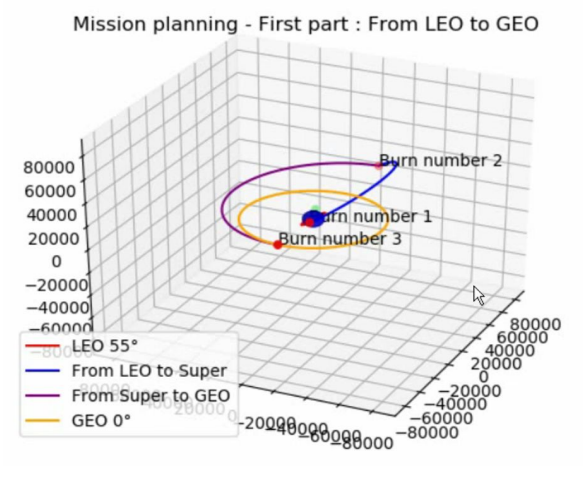
\includegraphics[width=0.6\linewidth]{mission1}
	\caption{Mission planning - First part}
\end{figure}
\textbf{\underline{Phase 2}} :
\begin{itemize}
	\item $\Delta v = 1.57$ km/s
\end{itemize}
{\underline{Further secondary burns}} :
\begin{itemize}
	\item Steering, rotation : $\approx 80$ m/s
	\item Reserve, correction : $\approx 200$ m/s
	\item Capture : $\approx 100$ m/s
\end{itemize}
\underline{\textbf{Total $\Delta v$ for the whole mission}} : $6.61$ km/s
\clearpage
{\underline{Phase 2 savings}} :
\begin{itemize}
	\item Aerobrake : $\approx 390$ m/s
	\item Inclination change during aerobrake : $1470$ m/s
\end{itemize}
\underline{\textbf{Total savings in both phases}} : $2.95$ km/s\\

\autoref{figtim2} shows the paths of the second part of the mission. Here only one exemplary aerobrake orbit is shown as a simplification.
\begin{figure}[H]
	\centering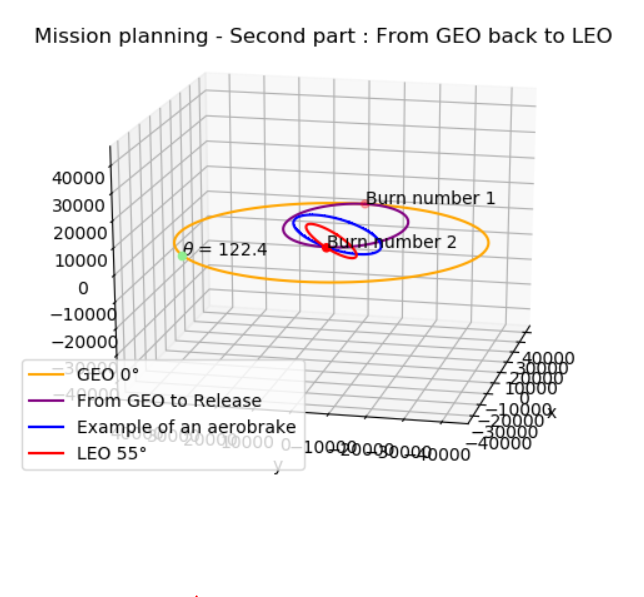
\includegraphics[width=0.7\linewidth]{mission2}
	\caption{Mission planning - Second part}\label{figtim2}
\end{figure}